\documentclass[aspectratio=169, 11pt]{beamer}

% --- Packages & Setup ---
\usepackage[utf8]{inputenc}
\usepackage[T1]{fontenc}
\usepackage{xcolor}
\usepackage{booktabs}
\usepackage{array}
\usepackage{graphicx}
\usepackage{tikz}
\usetikzlibrary{calc,arrows.meta,positioning,shapes.geometric}

\graphicspath{{../}{./}}

% Try loading Open Sans; fallback if missing
\IfFileExists{opensans.sty}{\usepackage[default,scale=0.95]{opensans}}{}

% --- Branding Colors ---
\definecolor{amritaMaroon}{HTML}{A4123F}
\definecolor{maroonSoft}{HTML}{F6E3E9}
\definecolor{inkGray}{HTML}{3A3A3A}
\definecolor{goldAccent}{HTML}{C79A3A}

% --- Theme Setup ---
\usetheme{Madrid}
\usecolortheme[named=amritaMaroon]{structure}
\setbeamertemplate{navigation symbols}{}
\setbeamertemplate{footline}[frame number]

% node styles reused across diagrams
\tikzset{
  lbl/.style={circle, draw=amritaMaroon, thick, fill=maroonSoft, minimum size=1.05cm, font=\scriptsize, align=center},
  lblcenter/.style={circle, draw=amritaMaroon, very thick, fill=amritaMaroon, text=white, minimum size=1.15cm, font=\bfseries\scriptsize, align=center},
  edg/.style={-, thick, draw=inkGray},
  edgfaint/.style={-, draw=inkGray!35},
  edghi/.style={-, ultra thick, draw=amritaMaroon},
  stepbox/.style={rectangle, draw=amritaMaroon, thick, fill=maroonSoft, rounded corners=2pt, minimum width=3.4cm, minimum height=0.75cm, font=\footnotesize, align=center}
}

% small icon-in-circle helpers for the Applications slide
\newcommand{\iconGraph}{%

\begin{tikzpicture}
\node[circle, fill=amritaMaroon, minimum size=0.9cm] (bg) {};
\node[circle, fill=white, minimum size=0.11cm, inner sep=0pt] (a) at ($(bg.center)+(-0.18,0.15)$) {};
\node[circle, fill=white, minimum size=0.11cm, inner sep=0pt] (b) at ($(bg.center)+(0.18,0.15)$) {};
\node[circle, fill=white, minimum size=0.11cm, inner sep=0pt] (c) at ($(bg.center)+(0,-0.2)$) {};
\draw[white, thin] (a) -- (b) -- (c) -- (a);
\end{tikzpicture}}

\newcommand{\iconMagnify}{%

\begin{tikzpicture}
\node[circle, fill=amritaMaroon, minimum size=0.9cm] (bg) {};
\draw[white, thick] ($(bg.center)+(-0.05,0.1)$) circle (0.17cm);
\draw[white, thick, line cap=round] ($(bg.center)+(0.07,-0.02)$) -- ($(bg.center)+(0.27,-0.24)$);
\end{tikzpicture}}

\newcommand{\iconDNA}{%

\begin{tikzpicture}
\node[circle, fill=amritaMaroon, minimum size=0.9cm] (bg) {};
\draw[white, thick] ($(bg.center)+(-0.2,0.28)$) .. controls ($(bg.center)+(0.2,0.12)$) and ($(bg.center)+(-0.2,-0.12)$) .. ($(bg.center)+(0.2,-0.28)$);
\draw[white, thick] ($(bg.center)+(0.2,0.28)$) .. controls ($(bg.center)+(-0.2,0.12)$) and ($(bg.center)+(0.2,-0.12)$) .. ($(bg.center)+(-0.2,-0.28)$);
\end{tikzpicture}}

\newcommand{\iconLeaf}{%

\begin{tikzpicture}
\node[circle, fill=amritaMaroon, minimum size=0.9cm] (bg) {};
\draw[white, thick] ($(bg.center)+(0,-0.3)$) -- ($(bg.center)+(0,0.05)$);
\filldraw[white] ($(bg.center)+(0.02,0.2)$) ellipse[x radius=0.22cm, y radius=0.13cm, rotate=40];
\draw[amritaMaroon, thin] ($(bg.center)+(-0.13,0.11)$) -- ($(bg.center)+(0.17,0.29)$);
\end{tikzpicture}}

\begin{document}

% ============================================================
% FRAME: What is the WL Graph Kernel?
% ============================================================
\begin{frame}{What is the WL Graph Kernel?}
    \framesubtitle{Weisfeiler--Lehman (WL) Graph Kernel}
    \begin{columns}[c]
        \column{0.52\textwidth}
        \textbf{Main idea}
        \vspace{0.15cm}

        The WL graph kernel compares graphs by \textbf{iteratively capturing the
        labels of each node and its neighborhood}.

        \vspace{0.3cm}
        \begin{itemize}
            \item Every node starts with a simple label.
            \item Labels are repeatedly updated using neighboring labels.
            \item The resulting label patterns are turned into a
            feature vector used to measure \textbf{similarity between graphs}.
        \end{itemize}

        \column{0.44\textwidth}
        \centering
        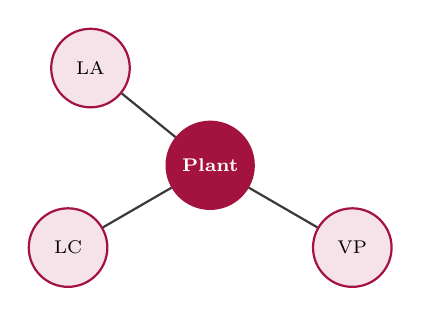
\begin{tikzpicture}[scale=0.95, every node/.style={transform shape}]
            \node[lblcenter] (p) at (0,0) {Plant};
            \node[lbl] (la) at (-1.6,1.3) {LA};
            \node[lbl] (lc) at (-1.9,-1.1) {LC};
            \node[lbl] (vp) at (1.9,-1.1) {VP};
            \draw[edg] (p) -- (la);
            \draw[edg] (p) -- (lc);
            \draw[edg] (p) -- (vp);
        \end{tikzpicture}

        \vspace{0.1cm}
        {\scriptsize\itshape A node's label evolves by absorbing
        information from its neighbors.}
    \end{columns}
\end{frame}

% ============================================================
% FRAME: How Does WL Work? (1/2) -- labels + aggregation
% ============================================================
\begin{frame}{How Does WL Work?}
    \begin{columns}[t]
        \column{0.48\textwidth}
        \textbf{1. Start with node labels}

        \vspace{0.1cm}
        {\footnotesize Each graph node has an initial label:}
        \begin{itemize}\footnotesize
            \item Plant $\rightarrow$ \texttt{plant}
            \item LA $\rightarrow$ \texttt{LA\_low}
            \item LC $\rightarrow$ \texttt{LC\_high}
            \item VP $\rightarrow$ \texttt{VP\_medium}
        \end{itemize}

        \vspace{0.25cm}
        \textbf{2. Iteratively aggregate neighborhood information}

        \vspace{0.1cm}
        {\footnotesize For each node:}

        \begin{center}
        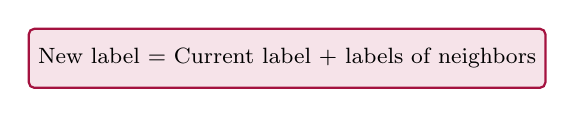
\begin{tikzpicture}
            \node[stepbox] {New label = Current label + labels of neighbors};
        \end{tikzpicture}
        \end{center}

        \column{0.48\textwidth}
        \centering
        {\footnotesize\textbf{Before}}\\[0.15cm]
        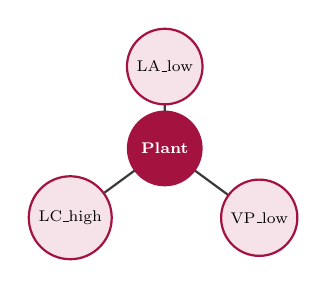
\begin{tikzpicture}[scale=0.8, every node/.style={transform shape}]
            \node[lbl] (la) at (0,1.3) {LA\_low};
            \node[lblcenter] (p) at (0,0) {Plant};
            \node[lbl] (lc) at (-1.5,-1.1) {LC\_high};
            \node[lbl] (vp) at (1.5,-1.1) {VP\_low};
            \draw[edg] (p) -- (la);
            \draw[edg] (p) -- (lc);
            \draw[edg] (p) -- (vp);
        \end{tikzpicture}

        \vspace{0.35cm}
        {\footnotesize\textbf{After WL iteration}}\\[0.1cm]
        {\scriptsize
        \begin{tabular}{@{}l@{}}
            Plant $\rightarrow$ plant \textbar\ LA\_low \textbar\ LC\_high \textbar\ VP\_low \\
            LA \quad\ $\rightarrow$ LA\_low \textbar\ plant \\
            LC \quad\ $\rightarrow$ LC\_high \textbar\ plant \\
            VP \quad\ $\rightarrow$ VP\_low \textbar\ plant \\
        \end{tabular}}
    \end{columns}

    \note{The main technique used in this research is the Weisfeiler--Lehman graph
    kernel. WL starts with the labels of the nodes and iteratively updates each
    node's label based on its own label and the labels of its neighbors.}
\end{frame}

% ============================================================
% FRAME: How Does WL Work? (2/2) -- feature vector + key point
% ============================================================
\begin{frame}{How Does WL Work? \textnormal{\footnotesize(contd.)}}
    \textbf{3. Build a feature representation}

    \vspace{0.05cm}
    {\footnotesize The labels generated at each WL iteration are counted to form
    a WL feature vector.}

    \vspace{0.08cm}
    \begin{center}
    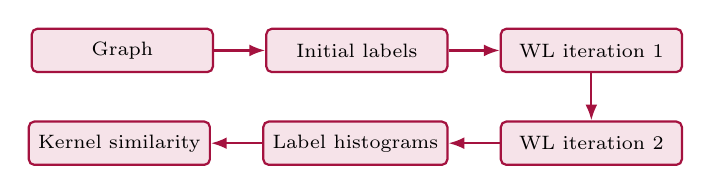
\begin{tikzpicture}[every node/.style={transform shape}]
        \tikzset{stepboxsm/.style={rectangle, draw=amritaMaroon, thick, fill=maroonSoft,
              rounded corners=2pt, minimum width=2.3cm, minimum height=0.55cm, font=\scriptsize, align=center}}
        \node[stepboxsm] (g)  {Graph};
        \node[stepboxsm, right=0.65cm of g] (il) {Initial labels};
        \node[stepboxsm, right=0.65cm of il] (i1) {WL iteration 1};
        \node[stepboxsm, below=0.6cm of i1] (i2) {WL iteration 2};
        \node[stepboxsm, left=0.65cm of i2] (lh) {Label histograms};
        \node[stepboxsm, left=0.65cm of lh] (ks) {Kernel similarity};
        \draw[-{Latex[length=2mm]}, thick, draw=amritaMaroon] (g) -- (il);
        \draw[-{Latex[length=2mm]}, thick, draw=amritaMaroon] (il) -- (i1);
        \draw[-{Latex[length=2mm]}, thick, draw=amritaMaroon] (i1) -- (i2);
        \draw[-{Latex[length=2mm]}, thick, draw=amritaMaroon] (i2) -- (lh);
        \draw[-{Latex[length=2mm]}, thick, draw=amritaMaroon] (lh) -- (ks);
    \end{tikzpicture}
    \end{center}

    \vspace{0.1cm}
    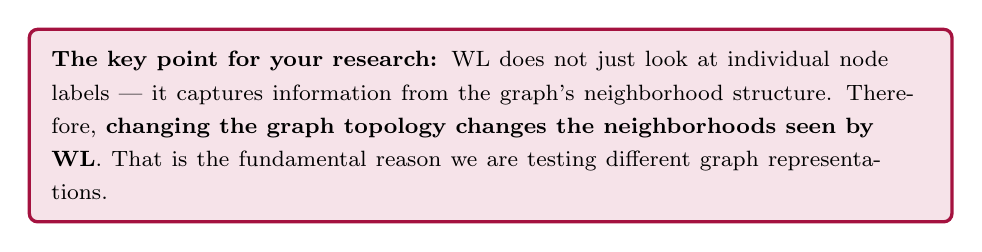
\begin{tikzpicture}
        \node[rectangle, draw=amritaMaroon, very thick, fill=maroonSoft,
              rounded corners=3pt, inner sep=8pt, text width=0.92\textwidth] {
            \footnotesize
            \textbf{The key point for your research:} WL does not just look at
            individual node labels --- it captures information from the graph's
            neighborhood structure. Therefore, \textbf{changing the graph
            topology changes the neighborhoods seen by WL}. That is the
            fundamental reason we are testing different graph representations.
        };
    \end{tikzpicture}

    \note{After several iterations, these labels are converted into a feature
    representation, which is then used to calculate similarity between graphs.
    Therefore, the neighborhood structure of a node directly affects the
    information extracted by WL. This gives us the motivation to investigate
    different graph topologies using exactly the same WL kernel.}
\end{frame}

% ============================================================
% FRAME: WL Algorithm -- Mathematical Formulation
% ============================================================
\begin{frame}{WL Algorithm: Mathematical Formulation}
    \framesubtitle{The formal update rule behind the visual picture}

    \begin{center}
        \Large
        $$ l_i(v) = f\left(l_{i-1}(v),\ \{\!\{\, l_{i-1}(u) : u \in N(v) \,\}\!\}\right) $$
    \end{center}

    \vspace{0.2cm}
    \begin{itemize}
        \item $l_i(v)$ -- the label of node $v$ after iteration $i$.
        \item $l_{i-1}(v)$ -- the node's own label from the previous iteration.
        \item $N(v)$ -- the set of neighbors of $v$.
        \item $\{\!\{\, l_{i-1}(u) : u \in N(v) \,\}\!\}$ -- the \textbf{multiset}
        of neighbor labels (order doesn't matter, repeats are kept).
        \item $f$ -- a hashing/compression function that combines a node's own
        label with its neighbors' labels into a new, compact label.
    \end{itemize}

    \vspace{0.15cm}
    {\footnotesize\itshape This is exactly the "current label + neighbor
    labels" update shown on the previous slide, written formally.}
\end{frame}

% ============================================================
% FRAME: Why Graph Representation Matters
% ============================================================
\begin{frame}{Why Graph Representation Matters}
    \framesubtitle{Same six traits, two different topologies}

    \begin{columns}[t]
        \column{0.48\textwidth}
        \centering
        {\footnotesize\textbf{Star graph}}\\[0.1cm]
        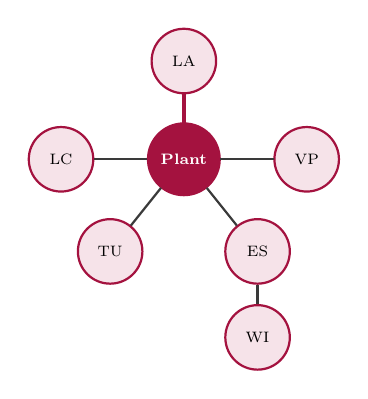
\begin{tikzpicture}[scale=0.78, every node/.style={transform shape}]
            \node[lbl] (la) at (0,1.6)   {LA};
            \node[lblcenter] (p) at (0,0) {Plant};
            \node[lbl] (lc) at (-2.0,0)  {LC};
            \node[lbl] (vp) at (2.0,0)   {VP};
            \node[lbl] (tu) at (-1.2,-1.5) {TU};
            \node[lbl] (es) at (1.2,-1.5)  {ES};
            \node[lbl] (wi) at (1.2,-2.9)  {WI};
            \draw[edghi] (p) -- (la);
            \draw[edg] (p) -- (lc);
            \draw[edg] (p) -- (vp);
            \draw[edg] (p) -- (tu);
            \draw[edg] (p) -- (es);
            \draw[edg] (es) -- (wi);
        \end{tikzpicture}

        \vspace{0.15cm}
        {\footnotesize LA sees only: \; LA $\rightarrow$ Plant}

        \column{0.48\textwidth}
        \centering
        {\footnotesize\textbf{Fully connected graph}}\\[0.1cm]
        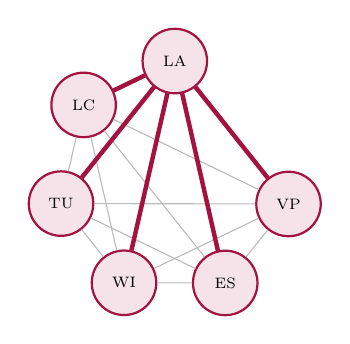
\begin{tikzpicture}[scale=0.78, every node/.style={transform shape}]
            \foreach \name/\ang in {LA/90, LC/141.4, TU/192.8, WI/244.2, ES/295.6, VP/347}
                \node[lbl] (\name) at (\ang:1.9) {\name};
            \foreach \a/\b in {LA/LC, LA/TU, LA/WI, LA/ES, LA/VP,
                               LC/TU, LC/WI, LC/ES, LC/VP,
                               TU/WI, TU/ES, TU/VP,
                               WI/ES, WI/VP, ES/VP}
                \draw[edgfaint] (\a) -- (\b);
            \foreach \b in {LC,TU,WI,ES,VP}
                \draw[edghi] (LA) -- (\b);
        \end{tikzpicture}

        \vspace{0.15cm}
        {\footnotesize LA sees all of: \; LA $\rightarrow$ LC, VP, TU, ES, WI}
    \end{columns}

    \vspace{0.3cm}
    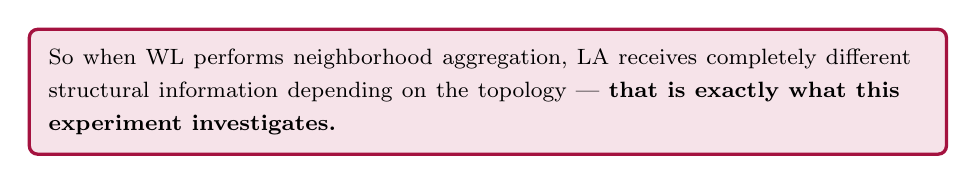
\begin{tikzpicture}
        \node[rectangle, draw=amritaMaroon, very thick, fill=maroonSoft,
              rounded corners=3pt, inner sep=7pt, text width=0.92\textwidth] {
            \footnotesize So when WL performs neighborhood aggregation, LA
            receives completely different structural information depending on
            the topology --- \textbf{that is exactly what this experiment
            investigates.}
        };
    \end{tikzpicture}
\end{frame}

% ============================================================
% FRAME: Where Are WL Graph Kernels Used? (Applications)
% ============================================================
\begin{frame}{Where Are WL Graph Kernels Used?}
    \framesubtitle{Applications of WL graph kernels}

    \footnotesize
    WL graph kernels are particularly useful when the input is naturally
    represented as graphs and the goal is to \textbf{classify or compare
    graph-structured data}.

    \vspace{0.4cm}
    \begin{columns}[T]
        \column{0.48\textwidth}
        \centering
        \iconGraph \\[4pt]
        \textbf{Graph Classification}\\[2pt]
        {\scriptsize\itshape Classify molecules, proteins, chemical
        compounds, etc.}

        \column{0.48\textwidth}
        \centering
        \iconMagnify \\[4pt]
        \textbf{Pattern Recognition}\\[2pt]
        {\scriptsize\itshape Identify structural patterns in graphs.}
    \end{columns}

    \vspace{0.55cm}
    \begin{columns}[T]
        \column{0.48\textwidth}
        \centering
        \iconDNA \\[4pt]
        \textbf{Bioinformatics}\\[2pt]
        {\scriptsize\itshape Compare molecular and biological structures.}

        \column{0.48\textwidth}
        \centering
        \iconLeaf \\[4pt]
        \textbf{Image / Plant Trait Analysis}\\[2pt]
        {\scriptsize\itshape Represent relationships among extracted
        features as graphs.}
    \end{columns}
\end{frame}

% ============================================================
% FRAME: Applications in the Literature (evidence slide)
% ============================================================
% \begin{frame}{Applications in the Literature}
%     \framesubtitle{WL graph kernels power real detection and comparison systems}
% 
%     \begin{center}
%     \begin{tikzpicture}[every node/.style={transform shape}]
%         \node[anchor=north west, inner sep=0] (img1) at (0,0)
%             {\includegraphics[width=3.5cm]{img1_malware.png}};
%         \node[anchor=north west, text width=7.7cm, align=left] (txt1) at (4.0,0.05) {
%             \footnotesize\textbf{Malware Detection}\\[2pt]
%             \scriptsize A \emph{contextual} WL graph kernel over program
%             behavior graphs distinguishes malware from benign software
%             (Narayanan et al., NTU Singapore).
%         };
% 
%         \node[anchor=north west, inner sep=0] (img2) at (0,-2.0)
%             {\includegraphics[width=3.5cm]{img2_program.png}};
%         \node[anchor=north west, text width=7.7cm, align=left] (txt2) at (4.0,-1.95) {
%             \footnotesize\textbf{Program Similarity Detection}\\[2pt]
%             \scriptsize The WL kernel compares program graphs directly to
%             detect similar or cloned code, without hand-crafted features
%             (Li, Saidi, Sanchez, Sch\"af \& Schweitzer).
%         };
% 
%         \node[anchor=north west, inner sep=0] (img3) at (0,-4.0)
%             {\includegraphics[width=3.5cm]{img3_bioinfo.png}};
%         \node[anchor=north west, text width=7.7cm, align=left] (txt3) at (4.0,-3.95) {
%             \footnotesize\textbf{Bioinformatics -- Protein Function}\\[2pt]
%             \scriptsize Amino-acid-level protein graphs, scored with WL
%             kernels, support \textbf{protein function} and phenotype
%             prediction -- the same principle used here for plant traits.
%         };
%     \end{tikzpicture}
%     \end{center}
% 
%     \vspace{0.05cm}
%     {\scriptsize\itshape Across security, software engineering, and biology,
%     the same idea recurs: represent structure as a graph, let WL capture
%     its neighborhoods, and compare.}
% \end{frame}

% ============================================================
% FRAME: How Does the WL Graph Kernel Perform Classification?
% ============================================================
\begin{frame}{How Does the WL Graph Kernel Perform Classification?}
    \framesubtitle{From plant graph to predicted class}

    \begin{center}
    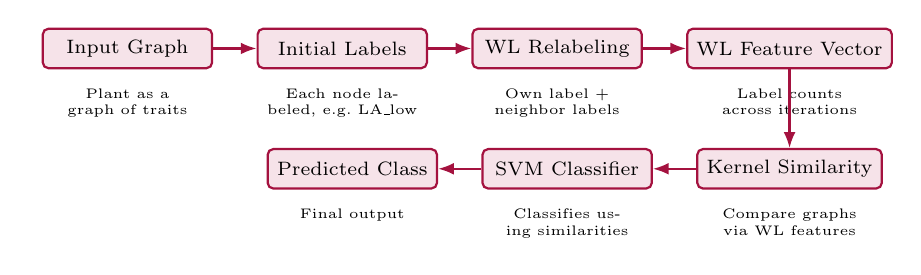
\begin{tikzpicture}[every node/.style={transform shape}]
        \tikzset{
            wlbox/.style={rectangle, draw=amritaMaroon, thick, fill=maroonSoft,
                rounded corners=2pt, minimum width=2.15cm, minimum height=0.5cm,
                font=\scriptsize, align=center},
            wlcap/.style={font=\tiny, align=center, text width=2.3cm}
        }
        % Row 1: left to right
        \node[wlbox] (b1) at (0,0) {Input Graph};
        \node[wlbox, right=0.55cm of b1] (b2) {Initial Labels};
        \node[wlbox, right=0.55cm of b2] (b3) {WL Relabeling};
        \node[wlbox, right=0.55cm of b3] (b4) {WL Feature Vector};

        \node[wlcap, below=0.12cm of b1] (c1) {Plant as a graph of traits};
        \node[wlcap, below=0.12cm of b2] (c2) {Each node labeled, e.g.\ LA\_low};
        \node[wlcap, below=0.12cm of b3] (c3) {Own label + neighbor labels};
        \node[wlcap, below=0.12cm of b4] (c4) {Label counts across iterations};

        % Row 2: right to left, continuing the flow
        \node[wlbox, below=1.0cm of b4] (b5) {Kernel Similarity};
        \node[wlbox, left=0.55cm of b5] (b6) {SVM Classifier};
        \node[wlbox, left=0.55cm of b6] (b7) {Predicted Class};

        \node[wlcap, below=0.12cm of b5] (c5) {Compare graphs via WL features};
        \node[wlcap, below=0.12cm of b6] (c6) {Classifies using similarities};
        \node[wlcap, below=0.12cm of b7] (c7) {Final output};

        \draw[-{Latex[length=2mm]}, thick, draw=amritaMaroon] (b1) -- (b2);
        \draw[-{Latex[length=2mm]}, thick, draw=amritaMaroon] (b2) -- (b3);
        \draw[-{Latex[length=2mm]}, thick, draw=amritaMaroon] (b3) -- (b4);
        \draw[-{Latex[length=2mm]}, thick, draw=amritaMaroon] (b4) -- (b5);
        \draw[-{Latex[length=2mm]}, thick, draw=amritaMaroon] (b5) -- (b6);
        \draw[-{Latex[length=2mm]}, thick, draw=amritaMaroon] (b6) -- (b7);
    \end{tikzpicture}
    \end{center}

    \vspace{0.1cm}
    \begin{center}
    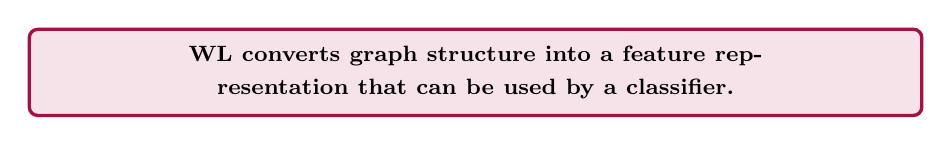
\begin{tikzpicture}
        \node[rectangle, draw=amritaMaroon, very thick, fill=maroonSoft,
              rounded corners=3pt, inner sep=6pt, text width=0.9\textwidth, align=center] {
            \footnotesize\textbf{WL converts graph structure into a feature
            representation that can be used by a classifier.}
        };
    \end{tikzpicture}
    \end{center}

    \vspace{0.12cm}
    \begin{center}
    {\scriptsize\itshape The topology determines which neighboring labels WL
    can see.}

    \vspace{0.1cm}
    {\footnotesize\bfseries Same traits + same WL kernel + different graph
    topology $\rightarrow$ different WL information $\rightarrow$ potentially
    different classification performance}
    \end{center}
\end{frame}

% ============================================================
% FRAME: Research Implementation Overview
% ============================================================
\begin{frame}{Research Implementation Overview}
    \framesubtitle{From raw images to a performance comparison}

    \begin{center}
    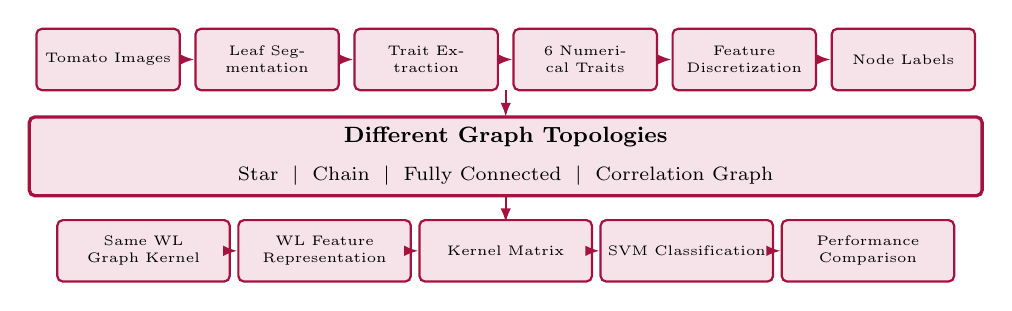
\begin{tikzpicture}[every node/.style={transform shape}]
        \tikzset{
            flowbox/.style={rectangle, draw=amritaMaroon, thick, fill=maroonSoft,
                rounded corners=2pt, text width=1.68cm, minimum height=0.78cm,
                inner sep=2pt, font=\tiny, align=center},
            flowarrow/.style={-{Latex[length=1.8mm]}, thick, draw=amritaMaroon}
        }

        % ---- Row 1: pre-processing chain ----
        \node[flowbox] (r1a) at (-5.05,0) {Tomato Images};
        \node[flowbox] (r1b) at (-3.03,0) {Leaf Segmentation};
        \node[flowbox] (r1c) at (-1.01,0) {Trait Extraction};
        \node[flowbox] (r1d) at (1.01,0)  {6 Numerical Traits};
        \node[flowbox] (r1e) at (3.03,0)  {Feature Discretization};
        \node[flowbox] (r1f) at (5.05,0)  {Node Labels};
        \foreach \a/\b in {r1a/r1b, r1b/r1c, r1c/r1d, r1d/r1e, r1e/r1f}
            \draw[flowarrow] (\a) -- (\b);

        % ---- connector into topology box ----
        \draw[flowarrow] (0,-0.39) -- (0,-0.73);

        % ---- Topology box ----
        \node[rectangle, draw=amritaMaroon, very thick, fill=maroonSoft,
              rounded corners=2pt, minimum width=12.1cm, minimum height=1.0cm,
              align=center] (topo) at (0,-1.23) {
            \footnotesize\textbf{Different Graph Topologies}\\[2pt]
            \scriptsize Star \;$\vert$\; Chain \;$\vert$\; Fully Connected
            \;$\vert$\; Correlation Graph
        };

        % ---- connector into row 2 ----
        \draw[flowarrow] (0,-1.73) -- (0,-2.07);

        % ---- Row 2: WL + classification chain ----
        \node[flowbox, text width=2.05cm] (r2a) at (-4.6,-2.43) {Same WL Graph Kernel};
        \node[flowbox, text width=2.05cm] (r2b) at (-2.3,-2.43) {WL Feature Representation};
        \node[flowbox, text width=2.05cm] (r2c) at (0,-2.43)     {Kernel Matrix};
        \node[flowbox, text width=2.05cm] (r2d) at (2.3,-2.43)  {SVM Classification};
        \node[flowbox, text width=2.05cm] (r2e) at (4.6,-2.43)  {Performance Comparison};
        \foreach \a/\b in {r2a/r2b, r2b/r2c, r2c/r2d, r2d/r2e}
            \draw[flowarrow] (\a) -- (\b);
    \end{tikzpicture}
    \end{center}

    \vspace{0.15cm}
    \begin{center}
    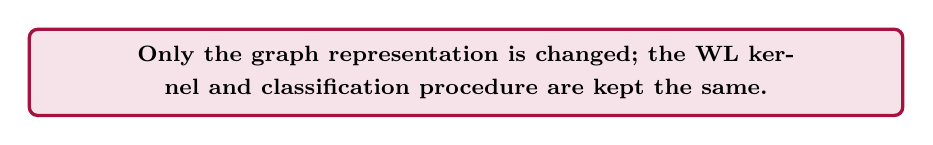
\begin{tikzpicture}
        \node[rectangle, draw=amritaMaroon, very thick, fill=maroonSoft,
              rounded corners=3pt, inner sep=6pt, text width=0.88\textwidth, align=center] {
            \footnotesize\textbf{Only the graph representation is changed; the
            WL kernel and classification procedure are kept the same.}
        };
    \end{tikzpicture}
    \end{center}

    \vspace{0.15cm}
    \begin{center}
    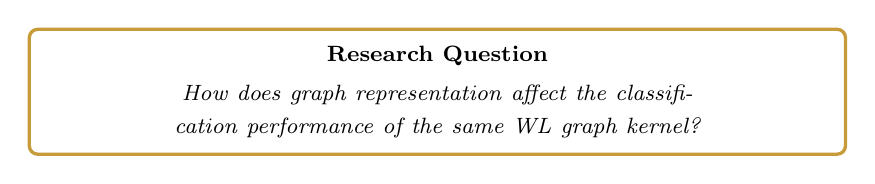
\begin{tikzpicture}
        \node[rectangle, draw=goldAccent, very thick, fill=white,
              rounded corners=3pt, inner sep=6pt, text width=0.82\textwidth, align=center] {
            \footnotesize\textbf{Research Question}\\[2pt]
            \footnotesize\itshape How does graph representation affect the
            classification performance of the same WL graph kernel?
        };
    \end{tikzpicture}
    \end{center}
\end{frame}

% ============================================================
% FRAME: Tomato Images -> Leaf Segmentation (before / after)
% ============================================================
\begin{frame}{From Tomato Images to Leaf Segmentation}
    \framesubtitle{Isolating the leaf from the background before trait extraction}

    \begin{center}
    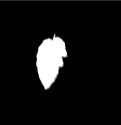
\includegraphics[width=0.85\linewidth, height=0.55\textheight, keepaspectratio]{segmentation_example.png}\\[0.1cm]
    {\scriptsize\itshape Raw leaf image $\rightarrow$ Segmentation $\rightarrow$ binary leaf mask}
    \end{center}

    \vspace{0.1cm}
    \footnotesize
    Before numerical traits can be extracted, each tomato leaf photo is
    segmented to separate the leaf from the background, producing a clean
    binary mask that isolates just the leaf region.
\end{frame}

% ============================================================
% FRAME: How Leaf Segmentation Works (algorithm steps)
% ============================================================
\begin{frame}{How Leaf Segmentation Works}
    \framesubtitle{From saturation threshold to a clean leaf mask}

    \begin{center}
    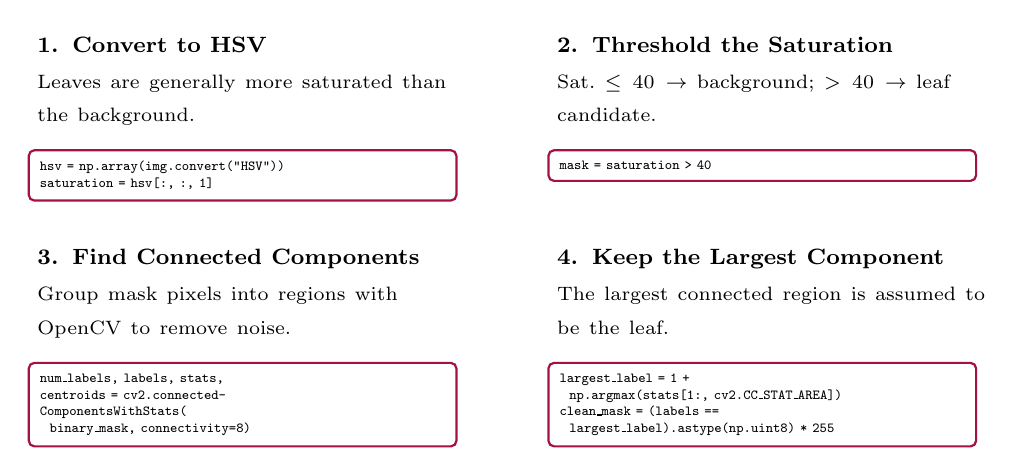
\begin{tikzpicture}[every node/.style={transform shape}]
        \tikzset{
            codebox/.style={rectangle, draw=amritaMaroon, thick, fill=white,
                rounded corners=2pt, text width=5.15cm, inner sep=4pt,
                align=left, font=\ttfamily\tiny, anchor=north west}
        }

        % --- Step 1 ---
        \node[anchor=north west, text width=5.5cm, align=left] (t1) at (-6.0,0) {
            \footnotesize\textbf{1. Convert to HSV}\\[1pt]
            \scriptsize Leaves are generally more saturated than the background.
        };
        \node[codebox] (c1) at (-6.0,-1.55) {
            hsv = np.array(img.convert("HSV"))\\
            saturation = hsv[:, :, 1]
        };

        % --- Step 2 ---
        \node[anchor=north west, text width=5.5cm, align=left] (t2) at (0.6,0) {
            \footnotesize\textbf{2. Threshold the Saturation}\\[1pt]
            \scriptsize Sat.\ $\leq 40 \rightarrow$ background;\ $> 40
            \rightarrow$ leaf candidate.
        };
        \node[codebox] (c2) at (0.6,-1.55) {
            mask = saturation > 40
        };

        % --- Step 3 ---
        \node[anchor=north west, text width=5.5cm, align=left] (t3) at (-6.0,-2.7) {
            \footnotesize\textbf{3. Find Connected Components}\\[1pt]
            \scriptsize Group mask pixels into regions with OpenCV to remove noise.
        };
        \node[codebox] (c3) at (-6.0,-4.25) {
            num\_labels, labels, stats,\\
            centroids = cv2.connected-\\
            ComponentsWithStats(\\
            \ \ binary\_mask, connectivity=8)
        };

        % --- Step 4 ---
        \node[anchor=north west, text width=5.5cm, align=left] (t4) at (0.6,-2.7) {
            \footnotesize\textbf{4. Keep the Largest Component}\\[1pt]
            \scriptsize The largest connected region is assumed to be the leaf.
        };
        \node[codebox] (c4) at (0.6,-4.25) {
            largest\_label = 1 +\\
            \ \ np.argmax(stats[1:, cv2.CC\_STAT\_AREA])\\
            clean\_mask = (labels ==\\
            \ \ largest\_label).astype(np.uint8) * 255
        };
    \end{tikzpicture}
    \end{center}

    \vspace{0.05cm}
    {\scriptsize\itshape The function finally returns \texttt{clean\_mask >
    0} -- a clean boolean mask isolating just the leaf.}
\end{frame}

% ============================================================
% FRAME: Feature Extraction from Segmented Leaves (overview tree)
% ============================================================
\begin{frame}{Feature Extraction from Segmented Leaves}
    \framesubtitle{Six image-derived traits, each capturing a different visual property}

    \footnotesize
    After segmentation, we extract \textbf{six image-derived traits} from the
    leaf region -- each one designed to capture a different visual property.

    \vspace{0.15cm}
    \begin{center}
    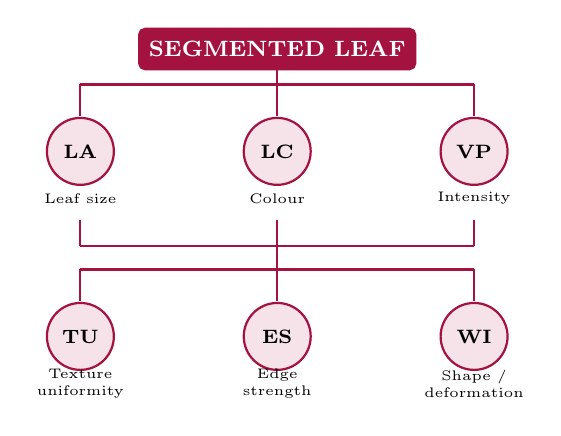
\begin{tikzpicture}[every node/.style={transform shape}]
        \tikzset{trait/.style={circle, draw=amritaMaroon, thick, fill=maroonSoft,
                 minimum size=0.85cm, font=\scriptsize\bfseries, align=center}}

        \node[rectangle, draw=amritaMaroon, very thick, fill=amritaMaroon,
              text=white, rounded corners=2pt, font=\footnotesize\bfseries,
              minimum width=3.2cm, minimum height=0.5cm] (leaf) at (0,0.55) {SEGMENTED LEAF};

        \draw[amritaMaroon, thick] (leaf.south) -- (0,0.1);
        \draw[amritaMaroon, thick] (-2.5,0.1) -- (2.5,0.1);
        \draw[amritaMaroon, thick] (-2.5,0.1) -- (-2.5,-0.3);
        \draw[amritaMaroon, thick] (0,0.1) -- (0,-0.3);
        \draw[amritaMaroon, thick] (2.5,0.1) -- (2.5,-0.3);

        \node[trait] (la) at (-2.5,-0.75) {LA};
        \node[trait] (lc) at (0,-0.75) {LC};
        \node[trait] (vp) at (2.5,-0.75) {VP};

        \node[font=\tiny, align=center] at (-2.5,-1.35) {Leaf size};
        \node[font=\tiny, align=center] at (0,-1.35) {Colour};
        \node[font=\tiny, align=center] at (2.5,-1.35) {Intensity};

        \draw[amritaMaroon, thick] (-2.5,-1.62) -- (-2.5,-1.95);
        \draw[amritaMaroon, thick] (0,-1.62) -- (0,-1.95);
        \draw[amritaMaroon, thick] (2.5,-1.62) -- (2.5,-1.95);
        \draw[amritaMaroon, thick] (-2.5,-1.95) -- (2.5,-1.95);
        \draw[amritaMaroon, thick] (0,-1.95) -- (0,-2.25);

        \draw[amritaMaroon, thick] (-2.5,-2.25) -- (2.5,-2.25);
        \draw[amritaMaroon, thick] (-2.5,-2.25) -- (-2.5,-2.65);
        \draw[amritaMaroon, thick] (0,-2.25) -- (0,-2.65);
        \draw[amritaMaroon, thick] (2.5,-2.25) -- (2.5,-2.65);

        \node[trait] (tu) at (-2.5,-3.1) {TU};
        \node[trait] (es) at (0,-3.1) {ES};
        \node[trait] (wi) at (2.5,-3.1) {WI};

        \node[font=\tiny, align=center] at (-2.5,-3.7) {Texture\\uniformity};
        \node[font=\tiny, align=center] at (0,-3.7) {Edge\\strength};
        \node[font=\tiny, align=center] at (2.5,-3.7) {Shape /\\deformation};
    \end{tikzpicture}
    \end{center}
\end{frame}

% ============================================================
% FRAME: From Traits to Graph Node Labels (pipeline + why six)
% ============================================================
\begin{frame}{From Traits to Graph Node Labels}
    \framesubtitle{Discretizing traits, and why we chose these six}

    \begin{center}
    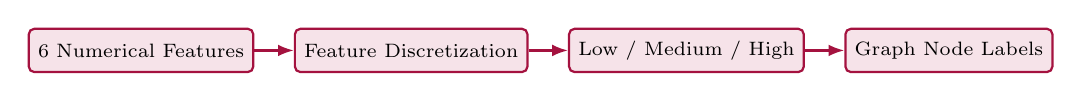
\begin{tikzpicture}[every node/.style={transform shape}]
        \tikzset{stepboxsm/.style={rectangle, draw=amritaMaroon, thick, fill=maroonSoft,
              rounded corners=2pt, minimum width=2.6cm, minimum height=0.55cm, font=\scriptsize, align=center}}
        \node[stepboxsm] (s1) {6 Numerical Features};
        \node[stepboxsm, right=0.5cm of s1] (s2) {Feature Discretization};
        \node[stepboxsm, right=0.5cm of s2] (s3) {Low / Medium / High};
        \node[stepboxsm, right=0.5cm of s3] (s4) {Graph Node Labels};
        \draw[-{Latex[length=2mm]}, thick, draw=amritaMaroon] (s1) -- (s2);
        \draw[-{Latex[length=2mm]}, thick, draw=amritaMaroon] (s2) -- (s3);
        \draw[-{Latex[length=2mm]}, thick, draw=amritaMaroon] (s3) -- (s4);
    \end{tikzpicture}
    \end{center}

    \vspace{0.35cm}
    \footnotesize\textbf{Why these six?} We deliberately capture \textbf{different
    visual characteristics} of the leaf, rather than six measurements of the
    same property:

    \vspace{0.25cm}
    \begin{center}
    \begin{tabular}{@{}ll@{\hspace{1.2cm}}ll@{}}
        \textbf{LA} & $\rightarrow$ size & \textbf{TU} & $\rightarrow$ texture \\[4pt]
        \textbf{LC} & $\rightarrow$ colour & \textbf{ES} & $\rightarrow$ edge / intensity structure \\[4pt]
        \textbf{VP} & $\rightarrow$ internal intensity variation & \textbf{WI} & $\rightarrow$ shape / boundary deformation \\
    \end{tabular}
    \end{center}
\end{frame}

% ============================================================
% FRAME: Feature Extraction Details (1/2) -- LA, LC, VP
% ============================================================
\begin{frame}{Feature Extraction Details (1/2)}
    \framesubtitle{Leaf Area, Leaf Colour, Vein Prominence}

    \begin{center}
    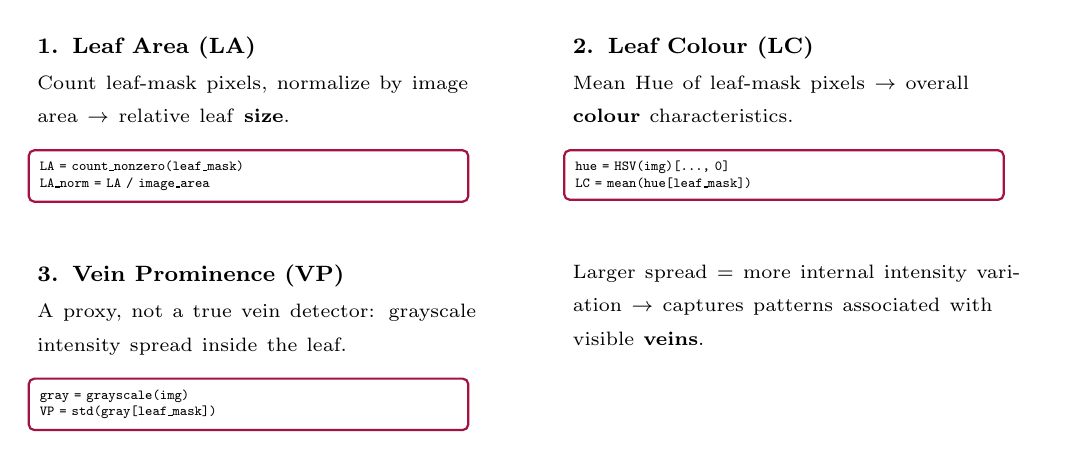
\begin{tikzpicture}[every node/.style={transform shape}]
        \tikzset{codebox2/.style={rectangle, draw=amritaMaroon, thick, fill=white,
                rounded corners=2pt, text width=5.3cm, inner sep=4pt,
                align=left, font=\ttfamily\tiny, anchor=north west}}

        \node[anchor=north west, text width=5.8cm, align=left] at (-6.1,0) {
            \footnotesize\textbf{1. Leaf Area (LA)}\\[1pt]
            \scriptsize Count leaf-mask pixels, normalize by image area
            $\rightarrow$ relative leaf \textbf{size}.
        };
        \node[codebox2] at (-6.1,-1.55) {
            LA = count\_nonzero(leaf\_mask)\\
            LA\_norm = LA / image\_area
        };

        \node[anchor=north west, text width=5.8cm, align=left] at (0.7,0) {
            \footnotesize\textbf{2. Leaf Colour (LC)}\\[1pt]
            \scriptsize Mean Hue of leaf-mask pixels $\rightarrow$ overall
            \textbf{colour} characteristics.
        };
        \node[codebox2] at (0.7,-1.55) {
            hue = HSV(img)[..., 0]\\
            LC = mean(hue[leaf\_mask])
        };

        \node[anchor=north west, text width=5.8cm, align=left] at (-6.1,-2.9) {
            \footnotesize\textbf{3. Vein Prominence (VP)}\\[1pt]
            \scriptsize A proxy, not a true vein detector: grayscale
            intensity spread inside the leaf.
        };
        \node[codebox2] at (-6.1,-4.45) {
            gray = grayscale(img)\\
            VP = std(gray[leaf\_mask])
        };

        \node[anchor=north west, text width=5.8cm, align=left] at (0.7,-2.9) {
            \scriptsize Larger spread $=$ more internal intensity variation
            $\rightarrow$ captures patterns associated with visible
            \textbf{veins}.
        };
    \end{tikzpicture}
    \end{center}
\end{frame}

% ============================================================
% FRAME: Feature Extraction Details (2/2) -- TU, ES, WI
% ============================================================
\begin{frame}{Feature Extraction Details (2/2)}
    \framesubtitle{Texture Uniformity, Edge Sharpness, Wilting Index}

    \begin{center}
    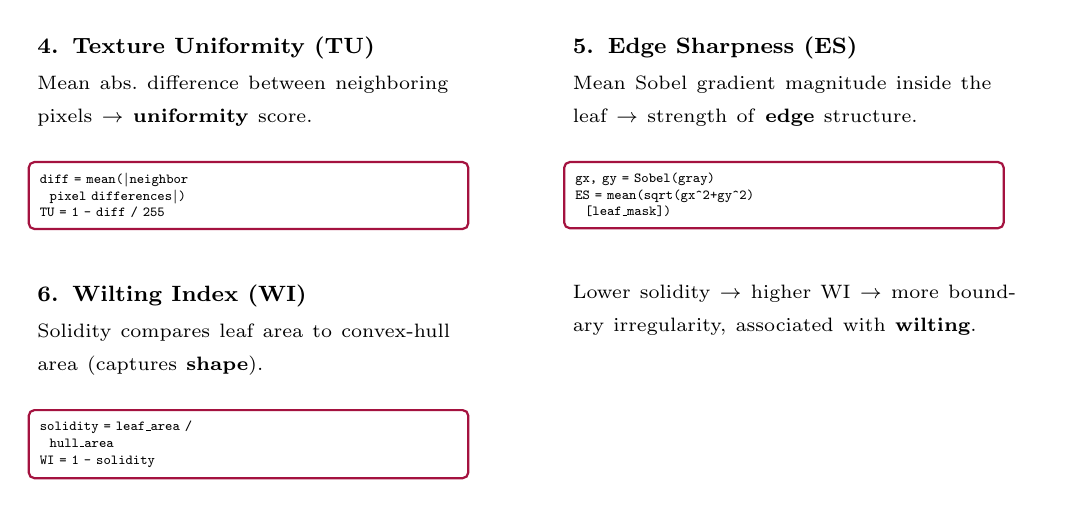
\begin{tikzpicture}[every node/.style={transform shape}]
        \tikzset{codebox2/.style={rectangle, draw=amritaMaroon, thick, fill=white,
                rounded corners=2pt, text width=5.3cm, inner sep=4pt,
                align=left, font=\ttfamily\tiny, anchor=north west}}

        \node[anchor=north west, text width=5.8cm, align=left] at (-6.1,0) {
            \footnotesize\textbf{4. Texture Uniformity (TU)}\\[1pt]
            \scriptsize Mean abs.\ difference between neighboring pixels
            $\rightarrow$ \textbf{uniformity} score.
        };
        \node[codebox2] at (-6.1,-1.7) {
            diff = mean(\textbar{}neighbor\\
            \ \ pixel differences\textbar{})\\
            TU = 1 - diff / 255
        };

        \node[anchor=north west, text width=5.8cm, align=left] at (0.7,0) {
            \footnotesize\textbf{5. Edge Sharpness (ES)}\\[1pt]
            \scriptsize Mean Sobel gradient magnitude inside the leaf
            $\rightarrow$ strength of \textbf{edge} structure.
        };
        \node[codebox2] at (0.7,-1.7) {
            gx, gy = Sobel(gray)\\
            ES = mean(sqrt(gx\textasciicircum{}2+gy\textasciicircum{}2)\\
            \ \ [leaf\_mask])
        };

        \node[anchor=north west, text width=5.8cm, align=left] at (-6.1,-3.15) {
            \footnotesize\textbf{6. Wilting Index (WI)}\\[1pt]
            \scriptsize Solidity compares leaf area to convex-hull area
            (captures \textbf{shape}).
        };
        \node[codebox2] at (-6.1,-4.85) {
            solidity = leaf\_area /\\
            \ \ hull\_area\\
            WI = 1 - solidity
        };

        \node[anchor=north west, text width=5.8cm, align=left] at (0.7,-3.15) {
            \scriptsize Lower solidity $\rightarrow$ higher WI $\rightarrow$
            more boundary irregularity, associated with \textbf{wilting}.
        };
    \end{tikzpicture}
    \end{center}
\end{frame}

% ============================================================
% FRAME: What we actually found (Dataset Overview)
% ============================================================
\begin{frame}{What We Actually Found}
    \framesubtitle{Dataset Overview}

    Our dataset contains \textbf{118 tomato-leaf images} across four classes:

    \vspace{0.3cm}
    \begin{itemize}
        \item \textbf{Healthy} --- 30
        \item \textbf{K deficiency} --- 29
        \item \textbf{N deficiency} --- 29
        \item \textbf{N + K deficiency} --- 30
    \end{itemize}

    \vspace{0.5cm}
    For every image, we extracted six features:
    $$ [LA_{norm}, LC, VP, TU, ES, WI] $$
\end{frame}

% ============================================================
% FRAME: Extracted Features & Summary Statistics
% ============================================================
\begin{frame}{Feature Summary Statistics}
    \framesubtitle{Overall values obtained across the dataset}

    \begin{table}
        \centering
        \scriptsize
        \begin{tabular}{@{}lrrrrl@{}}
            \toprule
            \textbf{Feature} & \textbf{Min} & \textbf{Max} & \textbf{Mean} & \textbf{Std} & \textbf{What we observed} \\
            \midrule
            \textbf{LA\_norm} & 0.0309 & 0.3091 & 0.0885 & 0.0438 & Considerable variation in leaf size \\
            \textbf{LC}       & 41.42  & 62.05  & 53.46  & 4.26   & Moderate colour variation \\
            \textbf{VP}       & 8.82   & 88.97  & 53.24  & 13.29  & Large variation in internal intensity \\
            \textbf{TU}       & 0.9449 & 0.9906 & 0.9703 & 0.0108 & Values are tightly concentrated \\
            \textbf{ES}       & 24.73  & 115.44 & 73.04  & 22.73  & Large variation in gradient/edge strength \\
            \textbf{WI}       & 0.0834 & 0.3739 & 0.1758 & 0.0692 & Noticeable variation in leaf shape irregularity \\
            \bottomrule
        \end{tabular}
    \end{table}
\end{frame}

% ============================================================
% FRAME: What this means for each feature (1/2)
% ============================================================
\begin{frame}{What This Means for Each Feature (1/2)}
    \footnotesize
    \begin{itemize}
        \item \textbf{1. LA --- Leaf Area}
        \begin{itemize}\scriptsize
            \item Values ranged from $\approx$ 0.031 to 0.309 after normalization.
            \item \textbf{Interpretation:} Substantial variation in relative size; provides useful variation between individual samples.
        \end{itemize}
        \vspace{0.25cm}
        
        \item \textbf{2. LC --- Leaf Colour}
        \begin{itemize}\scriptsize
            \item Mean Hue ranged from $\approx$ 41.4 to 62.1.
            \item \textbf{Interpretation:} Leaves don't all have the same colour characteristics; contains potentially useful information for distinguishing plant conditions.
        \end{itemize}
        \vspace{0.25cm}
        
        \item \textbf{3. VP --- Vein Prominence proxy}
        \begin{itemize}\scriptsize
            \item Fairly large spread ($\approx$ 8.8 to 89.0). Used grayscale standard deviation as a proxy for internal intensity variation (not an actual vein detector).
            \item \textbf{Interpretation:} Substantial variation in internal leaf appearance.
        \end{itemize}
    \end{itemize}
\end{frame}

% ============================================================
% FRAME: What this means for each feature (2/2)
% ============================================================
\begin{frame}{What This Means for Each Feature (2/2)}
    \footnotesize
    \begin{itemize}
        \item \textbf{4. TU --- Texture Uniformity}
        \begin{itemize}\scriptsize
            \item Values tightly concentrated ($\approx$ 0.945 to 0.991). Class means are quite close (K $\approx$ 0.9717, N $\approx$ 0.9716, N+K $\approx$ 0.9742).
            \item \textbf{Interpretation:} TU by itself does not appear to strongly separate the classes. However, not every feature needs to be highly discriminative individually; the WL representation can potentially use relationships between features.
        \end{itemize}
        \vspace{0.25cm}
        
        \item \textbf{5. ES --- Edge Sharpness proxy}
        \begin{itemize}\scriptsize
            \item Large variation ($\approx$ 24.7 to 115.4) using mean Sobel gradient magnitude.
            \item \textbf{Interpretation:} Different leaves show substantially different levels of intensity transitions and edge structures.
        \end{itemize}
        \vspace{0.25cm}
        
        \item \textbf{6. WI --- Wilting Index proxy}
        \begin{itemize}\scriptsize
            \item Proxy calculated as: $ WI = 1 - \frac{\text{leaf area}}{\text{convex hull area}} $
            \item \textbf{Interpretation:} Larger WI means a less-solid/more irregular leaf boundary. Noticeable variation ($\approx$ 0.083 to 0.374).
        \end{itemize}
    \end{itemize}
\end{frame}


% ============================================================
% FRAME: Feature Discretization & Node Label Generation (1/3)
% ============================================================
\begin{frame}{Feature Discretization}
    \framesubtitle{How numerical values become categorical labels}

    \textbf{1. Start with continuous feature values} \\
    \footnotesize For each plant, we have a numerical vector:
    $$ X = [LA_{norm}, LC, VP, TU, ES, WI] $$
    
    \vspace{0.3cm}
    \normalsize\textbf{2. Divide each feature into 3 levels} \\
    \footnotesize For each feature separately, we calculate two thresholds from the training data to avoid data leakage:

    \vspace{0.4cm}
    \begin{center}
    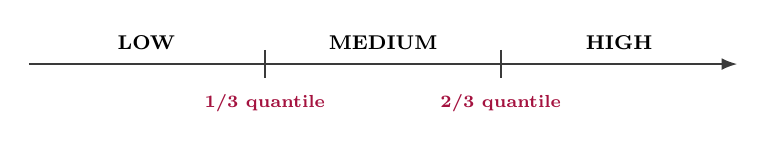
\begin{tikzpicture}[scale=0.9, every node/.style={transform shape}]
        % Main line
        \draw[thick, draw=inkGray, -{Latex[length=2mm]}] (0,0) -- (10,0);
        
        % Ticks
        \draw[thick, draw=inkGray] (3.33, 0.2) -- (3.33, -0.2) node[below=0.1cm, font=\scriptsize\bfseries, text=amritaMaroon] {1/3 quantile};
        \draw[thick, draw=inkGray] (6.66, 0.2) -- (6.66, -0.2) node[below=0.1cm, font=\scriptsize\bfseries, text=amritaMaroon] {2/3 quantile};
        
        % Labels
        \node[font=\footnotesize\bfseries] at (1.66, 0.3) {LOW};
        \node[font=\footnotesize\bfseries] at (5, 0.3) {MEDIUM};
        \node[font=\footnotesize\bfseries] at (8.33, 0.3) {HIGH};
    \end{tikzpicture}
    \end{center}

    \vspace{0.2cm}
    \begin{itemize}\scriptsize
        \item $< \text{1/3 quantile} \rightarrow \text{Low}$
        \item $\text{1/3 to} < \text{2/3 quantile} \rightarrow \text{Medium}$
        \item $\geq \text{2/3 quantile} \rightarrow \text{High}$
    \end{itemize}
\end{frame}

% ============================================================
% FRAME: Feature Discretization & Node Label Generation (2/3)
% ============================================================
\begin{frame}{Feature Discretization: Thresholds \& Example}
    
    \textbf{3. Our actual training thresholds}
    \begin{table}
        \centering
        \scriptsize
        \begin{tabular}{@{}lcc@{}}
            \toprule
            \textbf{Feature} & \textbf{Low / Medium boundary} & \textbf{Medium / High boundary} \\
            \midrule
            \textbf{LA\_norm} & 0.0666 & 0.0997 \\
            \textbf{LC}       & 52.1676 & 55.1118 \\
            \textbf{VP}       & 47.0985 & 54.2447 \\
            \textbf{TU}       & 0.9663 & 0.9777 \\
            \textbf{ES}       & 59.7588 & 85.5441 \\
            \textbf{WI}       & 0.1320 & 0.1927 \\
            \bottomrule
        \end{tabular}
    \end{table}

    \vspace{0.3cm}
    \textbf{4. Convert to WL node labels (Example Plant)}
    \begin{columns}
        \column{0.45\textwidth}
        \begin{itemize}\scriptsize
            \item LA = 0.0823 $\rightarrow$ \texttt{LA\_medium}
            \item LC = 54.31 $\rightarrow$ \texttt{LC\_medium}
            \item VP = 48.72 $\rightarrow$ \texttt{VP\_medium}
        \end{itemize}
        
        \column{0.45\textwidth}
        \begin{itemize}\scriptsize
            \item TU = 0.971 $\rightarrow$ \texttt{TU\_medium}
            \item ES = 91.4 $\rightarrow$ \texttt{ES\_high}
            \item WI = 0.154 $\rightarrow$ \texttt{WI\_medium}
        \end{itemize}
    \end{columns}
\end{frame}




\end{document}